Consider the two-dimensional region shown in Figure~\ref{fig:region}.
Inside this region, you will first
solve an electrostatic problem and then a quantum mechanics eigenvalue problem. Let the
region have length \(1\) in the \(x\) and \(y\) directions, given in dimensionless units.
The solid square in the interior has length \(0.25\) and height \(0.25\) and its center is
at \((x, y) = (0.625, 0.75)\). The circles at \((0.25, 0.125)\) and \((0.75, 0.125)\) are
point charges. Choose a two-dimensional grid to cover this region. You will need to
discretize the Laplacian on this grid and write a function to produce the result of applying
the discretized Laplacian to a vector, i.e., to the potential \(\phi(x, y)\) or the
wavefunction \(\psi(x, y)\) defined on this two-dimensional region. I recommend you choose a
grid of size \((N + 1) \times (N + 1)\), with the points with values of \(0\) or \((N + 1)\)
lying on the boundary. \(N = 128\) is a reasonable size to use.

\begin{figure}[hb]
    \centering
    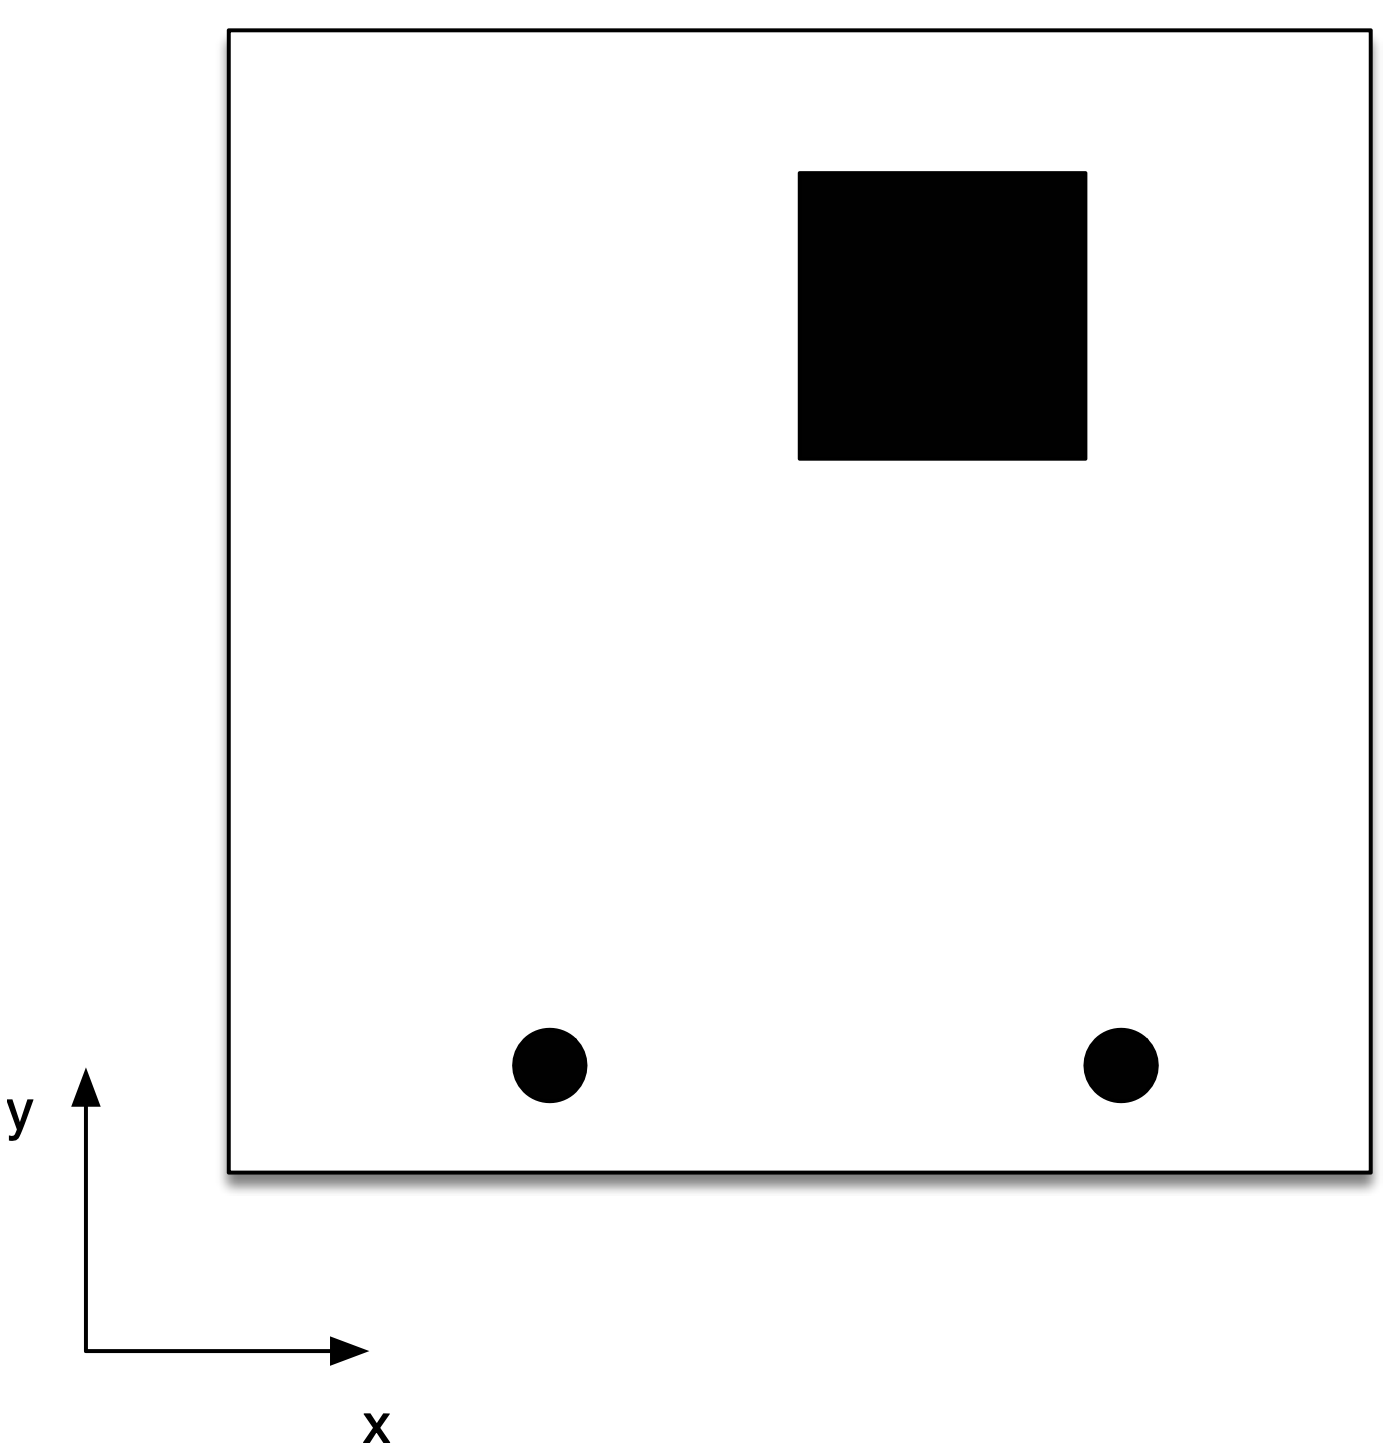
\includegraphics[width=0.5\textwidth]{region}
    \caption{A picture of the regions mentioned in the problems.}
    \label{fig:region}
\end{figure}

\section{Poisson's Equation}\label{sec:pe}

Write a program to use the conjugate gradient algorithm to solve Poisson's equation
%
\begin{equation}
    \nabla^2 \phi = -\rho
\end{equation}
%
(We will work in dimensionless units, so the \(a\) that enters the discretized Laplacian can be
set to \(1\) and the charges and potentials given will be in dimensionless units.) The
boundary of the region is held at a potential of zero, and the internal square is held at a
constant potential of \(5\). Let the point charges each have a value of \(20\), also in
dimensionless units. Thus you will want to solve the discretized version of Poisson's
equation with \(\rho(0.25, 0.125) = -20\) and \(\rho(0.75, 0.125) = -20\) and \(\rho = 0\)
everywhere else.

As discussed, one approach to this problem is to write your matrix
(discretized \(\nabla^2\)) times vector (\(\phi(x, y)\)) function for periodic boundary
conditions. Then before you return from the function, make sure the return value for
\(\mathrm{ A } x\) is set to the input value of \(x\) on the boundary of the region and for
the points on the interior square. For the conjugate gradient, you should set the initial
values for the solution \(x_0\) (or \(\phi(x, y)\)) to the potentials you're given. You also
want to make sure the initial residual \(r_0\) is zero on the boundary of the region and on
the internal square. This will ensure that the values of \(x\) have the correct boundary
conditions during the conjugate gradient.

You can do a simple test of your program by
removing the square from the above figure and putting the point charge in the center of the
large square region, i.e., \((0.5, 0.5)\). This will make the solution close to the known
analytical solution for a point charge without boundaries. (This should be the Coulomb
potential for a two-dimensional world, which has \(V(r) \sim -\ln r\), not the \(1/r\)
from our three-dimensional world.)

\subsection{The conjugate gradient method}

The conjugate gradient method


\begin{algorithm}
    \caption{The conjugate gradient method implementation of solving
        \(\mathrm{ A }\mathbf{ x } = \mathbf{ b }\).}
    \label{lst:cg}
    \begin{juliacode}
function solve(A, 𝐛, 𝐱₀=zeros(length(𝐛)); atol=eps(), maxiter=2000)
    history = ConvergenceHistory(maxiter, false, OffsetVector([], Origin(0)))
    𝐱ₙ = 𝐱₀
    𝐫ₙ = 𝐛 - A * 𝐱ₙ  # Initial residual, 𝐫₀
    𝐩ₙ = 𝐫ₙ  # Initial momentum, 𝐩₀
    for n in 0:maxiter
        if norm(𝐫ₙ) < atol
            history.isconverged = true
            break
        end
        αₙ = compute_alpha(A, 𝐫ₙ, 𝐩ₙ)
        𝐱ₙ₊₁ = 𝐱ₙ + αₙ * 𝐩ₙ
        𝐫ₙ₊₁ = 𝐫ₙ - αₙ * A * 𝐩ₙ
        βₙ = compute_beta(𝐫ₙ₊₁, 𝐫ₙ)
        𝐩ₙ₊₁ = 𝐫ₙ₊₁ + βₙ * 𝐩ₙ
        push!(history.data, IterationStep(n, αₙ, βₙ, 𝐱ₙ, 𝐫ₙ, 𝐩ₙ))
        # Prepare for a new iteration
        𝐱ₙ, 𝐫ₙ, 𝐩ₙ = 𝐱ₙ₊₁, 𝐫ₙ₊₁, 𝐩ₙ₊₁
    end
    return 𝐱ₙ, history
end
    \end{juliacode}
\end{algorithm}


\Question{} Plot the potential \(\phi(x, y)\) as a surface plot.
\newline
